\section{动力学参数的确定}


\begin{frame}{动力学参数}
    所谓动力学参数是指速率方程中所包含的参数，如吸附平衡常数，反应速率常数以及反应级数等。

    幂函数型动力学模型$(r=kc_\mathrm{A}^{\alpha}c_\mathrm{B}^{\beta})$需要确定：
    \begin{enumerate}
      \item 反应速率常数
      \item 反应级数
    \end{enumerate}
    双曲型动力学模型$r=\frac{k(p_{\mathrm{A}} p_{\mathrm{B}}-p_{\mathrm{R}} / K_{\mathrm{P}})}{(1+K_{\mathrm{A}} p_{\mathrm{A}}+K_{\mathrm{B}} p_{\mathrm{B}}+K_{\mathrm{R}} p_{\mathrm{R}})^{2}}$需要确定：
    \begin{enumerate}
      \item 反应速率常数
      \item 吸附平衡常数
    \end{enumerate}
\end{frame}


\begin{frame}{积分法求反应级数$\alpha$和反应速率常数$k$}
    积分法是将速率方程积分后，再对实验数据进行处理。例如，在恒容下进行的反应，速率方程用如下幂函数型方程表示：
    \begin{columns}[c]
        \column{10cm}
        $$r_\mathrm{A}=-\frac{\mathrm{d}c_\mathrm{A}}{\mathrm{d}t}=kc_\mathrm{A}^\alpha$$            
        $$\text{积分后为}\quad \frac{1}{c_{\mathrm{A}}^{\alpha-1}}-\frac{1}{c_{\mathrm{A} 0}^{\alpha-1}}=(\alpha-1) k t \quad(\alpha \neq 1)$$
        \column{4cm}
        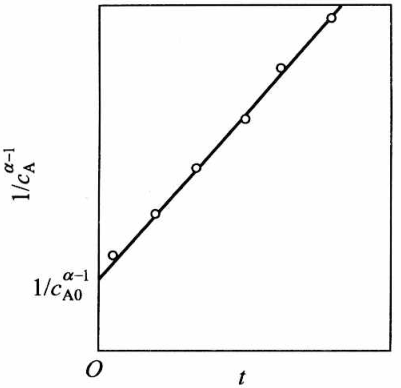
\includegraphics[height=2.7cm]{figs/fig2.6.png}
    \end{columns}        
        以时间$t$对$\frac{1}{c_{\mathrm{A}}^{\alpha-1}}$作图应得一直线，其斜率为$k(\alpha-1)$。但是$k$和$\alpha$均是要求的参数，都是未知值。因此，需先假定$\alpha$的值，根据实验测得的不同时间$t$时组分浓度$c_\mathrm{A}$的数据，按上述方法作图，若得一直线，表明所设$\alpha$值正确，否则需重新假定$\alpha$值，直到获得直线为止。
        \\还须指出，实验必须在等温下进行，这样才能保持$k$为常数。
\end{frame}


\begin{frame}{积分法求反应级数$\alpha$和反应速率常数$k$}
    \begin{table}        
        \caption{简单级数反应特征}
        \begin{tabular}{c l l l l}
            \Xhline{1pt}
            级数 & \makecell[c]{速率方程} & \makecell[c]{速率方程积分式} & \makecell[c]{线性关系} & \makecell[c]{$t$和$c_\mathrm{A}$关系}\\
            \hline
            \rule{0pt}{16pt} 1 & $r=kc_\mathrm{A}$ & $\ln c_\mathrm{A}=-kt+\ln c_\mathrm{A0}$ & $t\sim \ln c_\mathrm{A}$ & $t=\frac{1}{k}\ln\frac{c_\mathrm{A0}}{c_\mathrm{A}}$\\
            \rule{0pt}{16pt} 2 & $r=kc_\mathrm{A}^2$ & $\frac{1}{c_\mathrm{A}}=kt + \frac{1}{c_\mathrm{A0}}$ & $t\sim \frac{1}{c_\mathrm{A}}$ & $t=\frac{1}{k}(\frac{1}{c_\mathrm{A}}-\frac{1}{c_\mathrm{A0}})$ \\
            \rule{0pt}{16pt} 0 & $r=k$ & $c_\mathrm{A}=-kt+c_\mathrm{A0}$ & $t\sim c_\mathrm{A}$ & $t=\frac{1}{k}(c_\mathrm{A0}-c_\mathrm{A})$\\
            \Xhline{1pt}
        \end{tabular}        
\end{table}
\end{frame}


\begin{frame}{积分法求吸附平衡常数$K_\mathrm{A}$和反应速率常数$k$}
    又如速率方程
    $$r_\mathrm{A}=\frac{kK_\mathrm{A}p_\mathrm{A}}{1+K_\mathrm{A}p_\mathrm{A}}$$
    要用积分法求参数$k$和$K_\mathrm{A}$，需先将该式积分，但需首先确定反应速率$r_\mathrm{A}$的表示方式。若为气固相催化反应，常用$-\frac{\mathrm{d}F_\mathrm{A}}{\mathrm{d}W}$来表示，所以
    $$-\frac{\mathrm{d}F_\mathrm{A}}{\mathrm{d}W}=\frac{kK_\mathrm{A}p_\mathrm{A}}{1+K_\mathrm{A}p_\mathrm{A}}$$
    要积分上式，首先要把$F_\mathrm{A}$和$p_\mathrm{A}$变成转化率$X_\mathrm{A}$的函数。对于恒容过程，
    $$F_\mathrm{A}=F_\mathrm{A0}(1-X_\mathrm{A})$$
    $$p_\mathrm{A}=Py_\mathrm{A0}(1-X_\mathrm{A})$$
\end{frame}


\begin{frame}{积分法求吸附平衡常数$K_\mathrm{A}$和反应速率常数$k$}
    $$F_\mathrm{A0}\frac{\mathrm{d}X_\mathrm{A}}{\mathrm{d}W}=\frac{kK_\mathrm{A}Py_\mathrm{A0}(1-X_\mathrm{A})}{1+K_\mathrm{A}Py_\mathrm{A0}(1-X_\mathrm{A})}$$
    积分之，
    $$\int_0^W \frac{\mathrm{d}W}{F_\mathrm{A0}}= \int_0^{X_\mathrm{A}}\frac{1+K_\mathrm{A}Py_\mathrm{A0}(1-X_\mathrm{A})}{kK_\mathrm{A}Py_\mathrm{A0}(1-X_\mathrm{A})}\mathrm{d}X_\mathrm{A}$$
    $$\frac{W}{F_{\mathrm{A} 0}}=\frac{X_{\mathrm{A}}}{k}-\frac{\ln \left(1-X_{\mathrm{A}}\right)}{k K_{\mathrm{A}} P y_{\mathrm{A} 0}} \quad \text{或}\quad  \frac{W}{F_{\mathrm{A} 0} X_{\mathrm{A}}}=\frac{1}{k}-\frac{\ln \left(1-X_{\mathrm{A}}\right)}{k K_{\mathrm{A}} P y_{\mathrm{A} 0} X_{\mathrm{A}}}$$
    当压力、温度、起始气体组成以及催化剂用量一定情况下，改变$F_\mathrm{A0}$进行实验，分别测定相应转化率，根据所得数据，以$\ln(1-X_{\mathrm{A}})/X_{\mathrm{A}}$对$W/F_{\mathrm{A0}}X_{\mathrm{A}}$作图，可得一直线，斜率为$\frac{1}{kK_\mathrm{A}Py_\mathrm{A0}}$，截距为$1/k$,据此算出$k$和$K_{\mathrm{A}}$。    
\end{frame}


\begin{frame}{微分法求反应级数$\alpha$和反应速率常数$k$}
    微分法是根据不同实验条件下测得的反应速率，直接由速率方程估计参数值。仍以$r_\mathrm{A}=kc_\mathrm{A}^\alpha$为例，两边取对数则有
    $$\ln r_\mathrm{A}=\alpha \ln c_\mathrm{A} + \ln k$$
    根据实验数据，作$c_\mathrm{A} \sim t$曲线，在曲线上取若干点作切线求斜率，便得到不同时刻的$-\mathrm{d}c_\mathrm{A}/\mathrm{d}t$，即$r$。再以$\ln c_\mathrm{A}$对$\ln r_\mathrm{A}$作图，应得一直线，直线的斜率等于$\alpha$，截距等于$\ln k$。这样便可将参数值估算出来。
    \\也可以测定不同初始浓度时的初速率$r_0$，再以$\ln c_\mathrm{A}$对$\ln r_0$作图，求反应参数。因为在反应初始阶段，变化比较简单，复杂的因素较少。
\end{frame}


\begin{frame}{微分法求吸附平衡常数$K_\mathrm{A}$和反应速率常数$k$}
    又如速率方程
    $$r_\mathrm{A}=\frac{kK_\mathrm{A}p_\mathrm{A}}{1+K_\mathrm{A}p_\mathrm{A}}$$
    可改写成
    $$\frac{p_{\mathrm{A}}}{r_{\mathrm{A}}}=\frac{1}{k} p_{\mathrm{A}}+\frac{1}{k K_{\mathrm{A}}}$$
    以$\frac{p_{\mathrm{A}}}{r_{\mathrm{A}}}$对$p_{\mathrm{A}}$作图，得一直线，斜率为$1/k$，截距为$1/(kK_\mathrm{A})$。于是动力学参数$k$和$K_\mathrm{A}$可求定。
\end{frame}


\begin{frame}
    \frametitle{}
        \begin{figure}[htpb]
            \centering
            
\includegraphics[width=.9\linewidth]{2.10}
        \end{figure}
\end{frame}


\begin{frame}[t]
    \frametitle{}
    \begin{block}{例2.11}
        由实验测得镍催化剂上苯气相加氢反应的反应速率常数$k$及苯的吸附平衡常数$K_\mathrm{B}$与温度的关系如下表所示：
        \begin{table}
            \centering
            \begin{tabular}{ccccc}
                \bottomrule
                $T$(K) & 363 & 393 & 423 & 453\\ \hline
                $k$[\si{mol/(g.h.MPa^{1.5})}] & 14.52 & 25.96 & 45.07 & 66.03 \\ \hline
                $K_\mathrm{B}$(\si{MPa^{-1}}) & 1495 & 537.3 & 237.9 & 99.41\\  \toprule
            \end{tabular}
        \end{table}
        试求该反应的活化能及苯的吸附热。
        \tcblower
        提示：
        \[
            k = A\exp([-E/RT])
        \]
        \[
            K_\mathrm{B} = K_\mathrm{B0}\exp([q/RT])
        \]
    \end{block}
\end{frame}


\begin{frame}
    \frametitle{}
    \vspace{-0.5em}
    \begin{question}
        在铂催化剂上 ， 乙烯深度氧化的动力学方程可表示为
        \[
            r = \frac{kp_\mathrm{A}p_\mathrm{B}}{(1+K_\mathrm{B}p_\mathrm{B})^2}
        \]
        式中，$p_\mathrm{A}$、 $p_\mathrm{B}$分别为乙烯及氧的分压。在473K 等温下的实验数据如下表。试求该反应温度下的反应速率常数$k$和吸附平衡常数$K_\mathrm{B}$。
        \vspace{-0.5em}
        \begin{table}
            \centering
            \small
            \begin{tabular}{cccc||cccc}
                \bottomrule
                 & \begin{tabular}[c]{@{}c@{}}$p_\mathrm{A}\times 10^3$\\$\mathrm{MPa}$\end{tabular} & \begin{tabular}[c]{@{}c@{}}$p_\mathrm{B}\times 10^3$\\$\mathrm{MPa}$\end{tabular} & \begin{tabular}[c]{@{}c@{}}$r\times 10^4$\\$[\si{mol/(g.min)}]$\end{tabular} &  & \begin{tabular}[c]{@{}c@{}}$p_\mathrm{A}\times 10^3$\\$\mathrm{MPa}$\end{tabular} & \begin{tabular}[c]{@{}c@{}}$p_\mathrm{B}\times 10^3$\\$\mathrm{MPa}$\end{tabular} & \begin{tabular}[c]{@{}c@{}}$r\times 10^4$\\$[\si{mol/(g.min)}]$\end{tabular}\\ \hline
                1 & 8.99 & 3.23 & 0.672 & 7 & 7.75 & 1.82 & 0.828 \\ 
                2 & 14.22 & 3.00 & 1.072 & 8 & 6.17 & 1.73 & 0.656 \\ 
                3 & 8.86 & 4.08 & 0.598 & 9 & 6.13 & 1.73 & 0.694 \\ 
                4 & 8.32 & 2.03 & 0.713 & 10 & 6.98 & 1.56 & 0.791 \\ 
                5 & 4.37 & 0.89 & 0.610 & 11 & 2.87 & 1.06 & 0.418 \\ 
                6 & 7.75 & 1.74 & 0.834 &  &  &  &  \\ \toprule
            \end{tabular}
        \end{table}
        \vspace{-1.5em}
    \end{question}
\end{frame}